\chapter{\ifenglish Background Knowledge and Theory\else ทฤษฎีที่เกี่ยวข้อง\fi}

การทําโครงงานเริ่มต้นด้วยการศึกษาค้นคว้าทฤษฎีที่เกี่ยวข้อง หรืองานวิจัย/โครงงานที่เคยมีผู้พัฒนาและนําเสนอไว้แล้ว ซึ่งเนื้อหาในบทนี้ก็จะเกี่ยวกับ
การอธิบายถึงทฤษฎีที่นำไปประยุกต์ใช้กับโครงงานนี้ เพื่ออำนวยให้ผู้อ่านทำความเข้าใจกับตัวระบบของโครงงานได้ง่ายขึ้น

\section{You Only Look Once Object Detection Algorithm (YOLO)}
YOLO \cite{yolo} เป็นอัลกอริทึมสำหรับการระบุบริเวณที่สนใจภายในภาพ และจำแนกประเภทของวัตถุบนแต่ละบริเวณแบบเวลาจริงเหมือนกับตัวจำแนกภาพปกติ 
โดยที่ภาพหนึ่งสามารถประกอบด้วยบริเวณที่สนใจหลายบริเวณ แล้วแต่ละบริเวณจะนำไปจำแนกวัตถุที่แตกต่างกันได้ ซึ่งทำให้เกิดความซับซ้อนสูงในการ
จำแนกภาพระหว่างการตรวจจับวัตถุ ต่างจากอัลกอริทึมตรวจจับวัตถุทั่วไปที่จะใช้อัลกอริทึมแบบ Two-stage Object Detection YOLO 
นั้นจะใช้แบบ Single-shot Object Detection แทน ซึ่งใช้การสแกนภาพแต่ละภาพเพียงครั้งเดียวสำหรับการพยากรตำแหน่งของวัตถุที่ต้อง
การจะตรวจจับ และเนื่องจากการประมวลผลภาพเพียงครั้งเดียวนั้น ส่งผลให้อัลกอริทึมดังกล่าวใช้ระยะเวลาในการประมวลผลต่ำ 
เหมาะกับการนำไปใช้แบบเวลาจริง แต่ก็แลกมากับข้อเสียที่ความแม่นยำในการตรวจจับภาพนั้นอาจไม่มากเท่าอัลกอริทึมแบบ Two-stage Object Detection 
โดยใช้เทคนิคการเรียนรู้แบบ Convolutional Neural Network ดังรูปที่ 2.1
\begin{figure}[ht]
  \begin{center}
  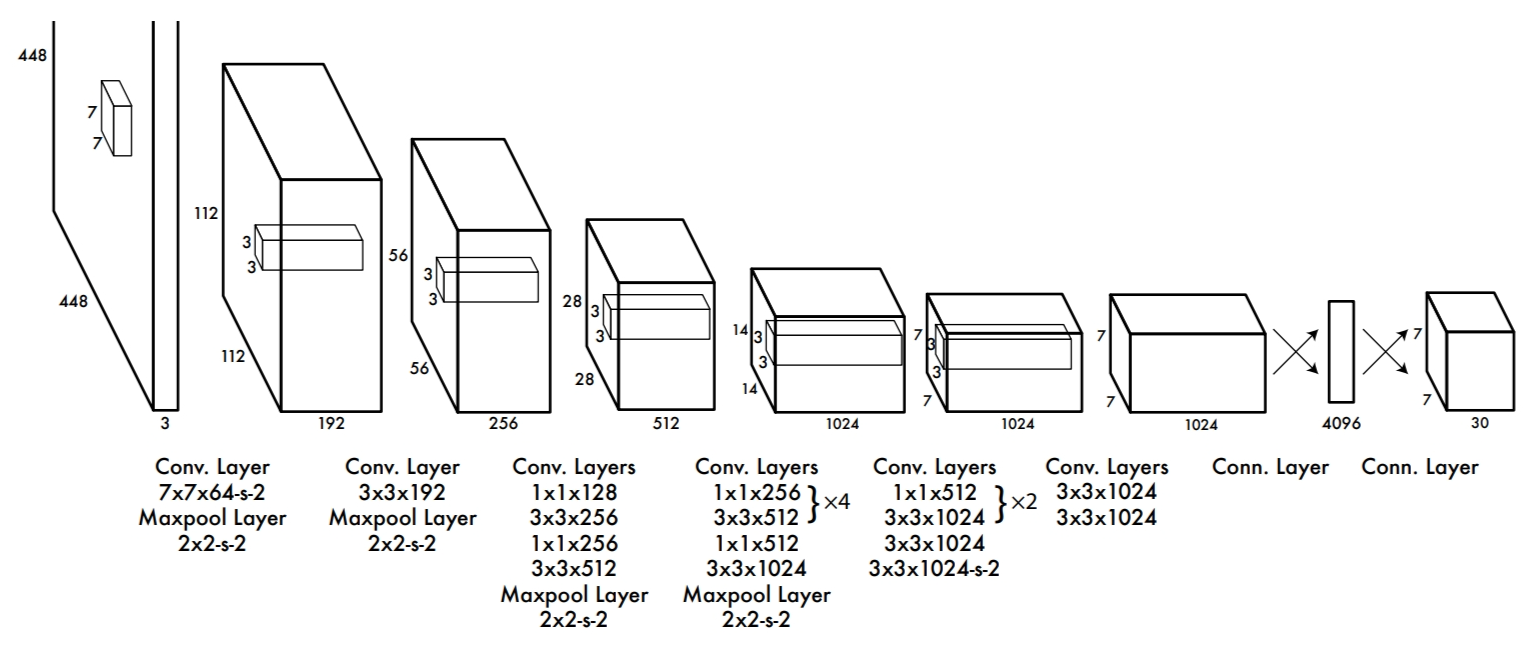
\includegraphics[scale=0.2]{resources/YOLO.png}
  \end{center}
  \caption[YOLO Architecture]{You Only Look Once Architecture}
  \label{fig:yolo architecture}
\end{figure}


\section{Object Relational Mapping (ORM)}
Object-Relational Mapping \cite{orm} เป็นการสร้างการสัมพันธ์ระหว่างฐานข้อมูลแบบ Relational กับโครงสร้างข้อมูลแบบ Object-Oriented 
ตามรูปที่ 2.2 ในการพัฒนาซอฟต์แวร์ เช่น เว็บแอปพลิเคชัน โดยที่ไม่ต้องเขียน SQL โดยตรงแต่สามารถใช้ภาษาโปรแกรมเพื่อจัดการกับข้อมูลแทน 
ซึ่งสามารถป้องกันการโจมตีแบบ SQL Injection ได้ ในกรณีที่กำหนดให้มีการเปลี่ยนแปลงในโครงสร้างข้อมูล 
คุณสมบัติหรือโครงสร้างข้อมูลในฐานข้อมูลจะถูกปรับเปลี่ยนตามในโครงสร้างของ Object ในโปรแกรม เป็นฐานข้อมูลแบบเสมือนในโปรแกรม 
โดยที่การจัดเก็บข้อมูลยังคงเป็นแบบ Relational เหมือนเดิม โดยไม่ต้องใช้ SQL Statements โดยตรง
\begin{figure}[ht]
  \begin{center}
  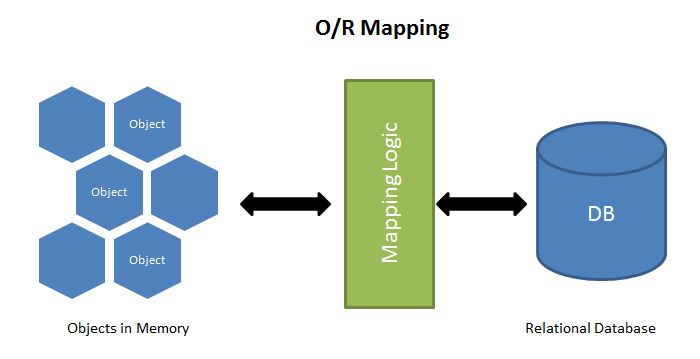
\includegraphics[scale=0.3]{resources/ORM.png}
  \end{center}
  \caption[Object Relational Mapping]{Object Relational Mapping}
  \label{fig:orm}
\end{figure}

\section{Hypertext Transfer Protocol (HTTP)}
HTTP (Hypertext Transfer Protocol) เป็นโปรโตคอลสื่อสารที่ใช้ในการส่งข้อมูลระหว่างเครื่องคอมพิวเตอร์บนเครือข่ายอินเทอร์เน็ต โดย HTTP 
มีหน้าที่เป็นตัวกลางในการร้องขอและส่งข้อมูลระหว่างเว็บไซต์ (web servers) และเบราว์เซอร์ (web browsers) หรือแอปพลิเคชันอื่น ๆ 
ที่ใช้เครือข่ายอินเทอร์เน็ต 
\begin{itemize}
  \item API (Application Programming Interface) เป็นชุดของกฎและโครงสร้างข้อมูลที่กำหนดโดยโปรแกรมคอมพิวเตอร์เพื่อให้แอปพลิเคชันอื่น ๆ 
  สามารถสื่อสารและทำงานร่วมกันได้ ในเชิงพื้นฐาน API เป็นวิธีที่แอปพลิเคชันใช้เรียกใช้ฟังก์ชันหรือการบริการที่ให้มาจากแหล่งข้อมูลหรือบริการ
  ซึ่งอาจเป็นเซิร์ฟเวอร์เว็บ ฐานข้อมูล หรือแหล่งข้อมูลอื่น ๆ โดยทั่วไป API จะรองรับการร้องขอและการตอบกลับโดยใช้ฟอแมตที่เป็นรูปแบบมาตรฐาน เช่น 
  JSON (JavaScript Object Notation) หรือ XML (Extensible Markup Language) 
\end{itemize}

\section{Docker}
Docker \cite{docker} เป็นเทคโนโลยีคอนเทนเนอร์แพลตฟอร์มที่ช่วยในการสร้างและทำการงานร่วมกับคอนเทนเนอร์อย่างมีประสิทธิภาพ ด้วย Docker 
ผู้ใช้สามารถแยกแยะและแพคเกจแอปพลิเคชันพร้อมกับสิ่งที่เกี่ยวข้องทั้งหมด เช่น ไฟล์ ระบบปฏิบัติการ ไลบรารี และสิ่งอื่น ๆ 
ลงในคอนเทนเนอร์ได้อย่างเรียบง่าย โดยมีโครงสร้างการทำงานตามรูปที่ 2.4 ผู้ใช้สามารถสร้าง และรันคอนเทนเนอร์ได้โดยง่าย นอกจากนี้ Docker 
ยังช่วยลดปัญหาเกี่ยวกับสภาพแวดล้อมและการติดตั้งโปรแกรมที่ซับซ้อน ทำให้การพัฒนาและการทำงานของโปรแกรมมีประสิทธิภาพมากขึ้น 
\begin{figure}[ht]
  \begin{center}
  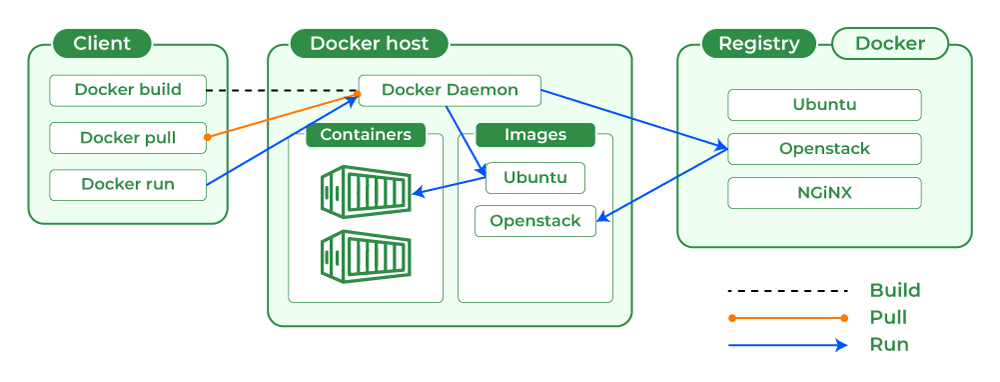
\includegraphics[scale=0.3]{resources/Docker.png}
  \end{center}
  \caption[Docker Architecture]{Docker Architecture}
  \label{fig:docker}
\end{figure}

\section{Interactive Website}
Interactive website \cite{interactive-web} คือ เว็บไซต์ที่สามารถให้ผู้ใช้งาน communicate หรือ interact เช่น การแสดงความคิดเห็น การตอบโต้กับตัวเว็บ 
การได้รับผลจากการกระทําในเว็บ ในลักษระที่เป็นมิตรต่อผู้ใช้ โดยปัจจุบัน มักใช้ animation sound picture audio etc. ประกอบ 
เพื่อให้มีความสนุกสนานและเพิ่มการเข้าถึงได้ง่ายของผู้ใช้ ทั้งนี้อาจทําเพื่อเก็บข้อมูลหลังจากการใช้งานเว็บไซต์ได้อีกด้วย ซึ่งดีกว่าเว็บที่มีแต่ตัวอักษร หรือ 
การแสดงผลเฉย ๆ ที่ได้รับข้อมูลทางฝ่ายเดียวอย่างแน่นอน

\section{Azure Public Cloud}
Azure Public Cloud \cite{azure} เป็นแพลตฟอร์มคลาวด์คอมพิวติ้งที่พัฒนาโดย Microsoft ซึ่งให้บริการหลากหลายประเภท เช่น การประมวลผล (compute), การจัดเก็บข้อมูล (storage), การเครือข่าย (networking), และการวิเคราะห์ข้อมูล (analytics) โดย Azure Public Cloud ช่วยให้องค์กรและนักพัฒนาสามารถสร้างและจัดการแอปพลิเคชันได้อย่างมีประสิทธิภาพและยืดหยุ่น

Azure Public Cloud มีบริการที่หลากหลาย เช่น:
\begin{itemize}
  \item \textbf{Azure Virtual Machines (VMs)}: บริการที่ช่วยให้ผู้ใช้สามารถสร้างและจัดการเครื่องเสมือนบนคลาวด์ได้
  \item \textbf{Azure App Services}: บริการที่ช่วยในการพัฒนาและโฮสต์เว็บแอปพลิเคชันและ API บนคลาวด์
  \item \textbf{Azure Storage}: บริการจัดเก็บข้อมูลที่มีความยืดหยุ่นและสามารถขยายขนาดได้ตามความต้องการ
  \item \textbf{Azure SQL Database}: บริการฐานข้อมูลเชิงสัมพันธ์ที่มีความเสถียรและปลอดภัย
  \item \textbf{Azure Kubernetes Service (AKS)}: บริการที่ช่วยในการจัดการและปรับใช้คอนเทนเนอร์โดยใช้ Kubernetes
\end{itemize}

Azure Public Cloud ยังมีความสามารถในการรองรับการทำงานร่วมกับเครื่องมือและเทคโนโลยีอื่น ๆ เช่น Docker, Kubernetes, และ DevOps ซึ่งช่วยให้การพัฒนาและการจัดการแอปพลิเคชันเป็นไปอย่างราบรื่นและมีประสิทธิภาพ

\section{Role-Based Access Control (RBAC)}
Role-Based Access Control (RBAC) \cite{rbac} เป็นวิธีการจัดการสิทธิ์การเข้าถึงระบบที่กำหนดสิทธิ์การเข้าถึงตามบทบาทของผู้ใช้ในองค์กร โดย RBAC ช่วยให้การจัดการสิทธิ์การเข้าถึงเป็นไปอย่างมีประสิทธิภาพและปลอดภัยมากขึ้น เนื่องจากสิทธิ์การเข้าถึงจะถูกกำหนดตามบทบาทที่ผู้ใช้มีในองค์กร ไม่ใช่ตามผู้ใช้แต่ละคน

RBAC มีองค์ประกอบหลักดังนี้:
\begin{itemize}
  \item \textbf{Roles (บทบาท)}: บทบาทที่กำหนดสิทธิ์การเข้าถึงตามหน้าที่หรือความรับผิดชอบของผู้ใช้ในองค์กร
  \item \textbf{Permissions (สิทธิ์)}: สิทธิ์การเข้าถึงที่กำหนดให้กับบทบาทต่าง ๆ เช่น การอ่าน การเขียน หรือการลบข้อมูล
  \item \textbf{Users (ผู้ใช้)}: ผู้ใช้ที่ได้รับการกำหนดบทบาทและสิทธิ์การเข้าถึงตามบทบาทนั้น ๆ
  \item \textbf{Sessions (เซสชัน)}: การเชื่อมต่อระหว่างผู้ใช้และระบบที่กำหนดสิทธิ์การเข้าถึงตามบทบาทของผู้ใช้ในช่วงเวลาหนึ่ง
\end{itemize}

RBAC ช่วยลดความซับซ้อนในการจัดการสิทธิ์การเข้าถึงและเพิ่มความปลอดภัยในการเข้าถึงระบบ โดยเฉพาะในองค์กรที่มีผู้ใช้จำนวนมากและมีการเปลี่ยนแปลงบทบาทของผู้ใช้อยู่บ่อยครั้ง

\section{Json Web Token (JWT)}
JSON Web Token (JWT) \cite{jwt} เป็นมาตรฐานเปิด (RFC 7519) ที่กำหนดวิธีการสร้างโทเค็นที่ใช้ในการส่งข้อมูลระหว่างฝ่ายต่าง ๆ อย่างปลอดภัยในรูปแบบของ JSON โดย JWT ประกอบด้วยสามส่วนหลัก ๆ คือ Header, Payload และ Signature ซึ่งถูกเข้ารหัสและเชื่อมต่อกันด้วยจุด (.) เพื่อสร้างโทเค็นที่สมบูรณ์

JWT มีการใช้งานที่หลากหลาย เช่น:
\begin{itemize}
  \item \textbf{Authentication (การยืนยันตัวตน)}: JWT ถูกใช้ในการยืนยันตัวตนของผู้ใช้ในระบบ โดยโทเค็นจะถูกส่งไปยังผู้ใช้หลังจากที่ผู้ใช้ทำการล็อกอินสำเร็จ และผู้ใช้จะต้องส่งโทเค็นนี้กลับมาในคำขอถัดไปเพื่อยืนยันตัวตน
  \item \textbf{Information Exchange (การแลกเปลี่ยนข้อมูล)}: JWT สามารถใช้ในการส่งข้อมูลระหว่างฝ่ายต่าง ๆ อย่างปลอดภัย เนื่องจากข้อมูลในโทเค็นถูกเข้ารหัสและสามารถตรวจสอบความถูกต้องได้
\end{itemize}

JWT มีข้อดีหลายประการ เช่น:
\begin{itemize}
  \item \textbf{Compact (กระชับ)}: โทเค็นมีขนาดเล็กและสามารถส่งผ่าน URL, POST parameters หรือใน HTTP headers ได้อย่างง่ายดาย
  \item \textbf{Self-contained (บรรจุข้อมูลในตัวเอง)}: โทเค็นประกอบด้วยข้อมูลที่จำเป็นทั้งหมด เช่น ข้อมูลผู้ใช้และสิทธิ์การเข้าถึง ทำให้ไม่จำเป็นต้องเข้าถึงฐานข้อมูลในทุกคำขอ
\end{itemize}

\section{Microservices Architecture}
Microservices Architecture \cite{microservices} เป็นสถาปัตยกรรมในการออกแบบระบบซอฟต์แวร์ ที่แบ่งแอปพลิเคชันออกเป็นบริการขนาดเล็ก ๆ ที่สามารถพัฒนา ทดสอบ และปรับใช้ได้อย่างอิสระ โดยแต่ละบริการจะทำงานร่วมกันผ่าน API และสามารถสื่อสารกันได้ผ่านโปรโตคอลต่าง ๆ เช่น HTTP หรือ AMQP

ข้อดีของ Microservices Architecture ได้แก่:
\begin{itemize}
  \item \textbf{Scalability (การขยายขนาด)}: สามารถขยายขนาดบริการแต่ละตัวได้อย่างอิสระตามความต้องการของระบบ
  \item \textbf{Flexibility (ความยืดหยุ่น)}: สามารถใช้เทคโนโลยีและภาษา.ในการเขียนโปรแกรมที่แตกต่างกันในแต่ละเซอร์วิสโดยที่ไม่มีผลกระทบต่อระบบโดยรวม
  \item \textbf{Resilience (ความทนทาน)}: หากบริการใดบริการหนึ่งล้มเหลว จะไม่ส่งผลกระทบต่อบริการอื่น ๆ ในระบบ
  \item \textbf{Continuous Deployment (การปรับใช้อย่างต่อเนื่อง)}: สามารถปรับใช้และอัปเดตบริการแต่ละตัวได้อย่างรวดเร็วและง่ายดาย
\end{itemize}

\section{Cross Platform}
Cross Platform \cite{crossplatform} เป็นแนวคิดในการพัฒนาแอปพลิเคชันที่สามารถทำงานได้บนหลายแพลตฟอร์ม เช่น iOS, Android, และ Windows โดยใช้โค้ดเบสเดียวกัน ซึ่งช่วยลดเวลาและค่าใช้จ่ายในการพัฒนาและบำรุงรักษาแอปพลิเคชัน

ข้อดีของ Cross Platform ได้แก่:
\begin{itemize}
  \item \textbf{Code Reusability (การใช้โค้ดซ้ำ)}: สามารถใช้โค้ดเบสเดียวกันในการพัฒนาแอปพลิเคชันสำหรับหลายแพลตฟอร์ม
  \item \textbf{Cost Efficiency (ประหยัดค่าใช้จ่าย)}: ลดค่าใช้จ่ายในการพัฒนาและบำรุงรักษาแอปพลิเคชัน
  \item \textbf{Faster Time-to-Market (เวลาสู่ตลาดเร็วขึ้น)}: สามารถเปิดตัวแอปพลิเคชันได้เร็วขึ้นเนื่องจากไม่ต้องพัฒนาแยกกันสำหรับแต่ละแพลตฟอร์ม
  \item \textbf{Consistency (ความสม่ำเสมอ)}: ให้ประสบการณ์การใช้งานที่สม่ำเสมอบนทุกแพลตฟอร์ม
\end{itemize}

เครื่องมือที่นิยมใช้ในการพัฒนาแอปพลิเคชันแบบ Cross Platform ได้แก่ Flutter, React Native, และ Xamarin